\documentclass[10pt,a4paper]{article}
\usepackage[margin=2.2cm]{geometry}
\usepackage[T1]{fontenc}
\usepackage{lmodern,microtype,amsmath,amssymb,graphicx,booktabs,array,xcolor,tabularx,multirow,enumitem}
\usepackage{listings}
\usepackage{tikz}
\usetikzlibrary{positioning,arrows.meta,fit}
\usepackage[colorlinks,linkcolor=blue!50!black,urlcolor=blue!50!black,citecolor=blue!50!black]{hyperref}
\lstset{basicstyle=\ttfamily\footnotesize,columns=fullflexible,keepspaces,frame=single,framerule=0.3pt,
  rulecolor=\color{black!30},backgroundcolor=\color{black!3},breaklines,showstringspaces=false,
  commentstyle=\color{black!55},morecomment=[l]{\#},xleftmargin=2pt,xrightmargin=2pt}
\newcommand{\code}[1]{\texttt{\detokenize{#1}}}
\setlist{itemsep=1pt,topsep=3pt}
\title{The Sahyadri simulation manager on pawna:\\ running, checking and archiving many simulations}
\author{Sahyadri collaboration --- prepared with Claude Code}
\date{13 November 2026 \\[2pt] \small repository \code{a-paranjape/sahyadri-sandbox}, branch \code{run-manager}}

\begin{document}
\maketitle

\begin{abstract}
The Sahyadri suite needs many $N$-body simulations (several cosmologies, many realisations, up to $2048^3$
particles), each followed by halo finding, merger trees, halo environment tables and FITS conversion. A
$2048^3$ run writes about 9\,TB of snapshots, more than can be kept. This report describes the run manager
built on the branch \code{run-manager}. It runs on the pawna head node and drives the
pipeline pkdgrav3 $\to$ Rockstar $\to$ consistent-trees $\to$ vahc $\to$ FITS for every registered run. It
queues simulations within limits you set, restarts them from checkpoints when they reach the wall time, and runs
Rockstar in batches while the simulation is still going. It then verifies every product, including the matter
power spectrum against CLASS, and archives the kept data to \code{/storage} with checksums read back from disk.
The working copy is deleted only after you approve it, in two steps. A web page, reached from a laptop through an
ssh tunnel, shows every run and has the controls. The manager was tested on nine $64^3$ runs, two $128^3$ runs
and one $512^3$ run, all of which went through to the archive. The tests found and fixed fourteen problems, listed in Section~\ref{sec:bugs}.
\end{abstract}

\tableofcontents

\section{Why a manager}

A Sahyadri production run is a chain of PBS jobs: the pkdgrav3 simulation, Rockstar, consistent-trees, the halo
environment tables (vahc, tens, vpot), and the conversion to FITS. Until now each chain was submitted by hand with
\code{submit_pipeline.sh}, as one \code{afterok} chain whose Rockstar job waited for the whole simulation. For a
suite of many runs this has four problems.

\begin{itemize}
  \item \textbf{Space.} A $2048^3$ run with 101 outputs writes about 9\,TB of snapshots (10.5 bytes per particle
    per output, measured at $128^3$ and $512^3$). Only a few full snapshots, a 1\,\% subsample of the others and
    the halo products are meant to be kept. Something has to decide when the rest may go, and has to check
    first that the kept part is safely elsewhere.
  \item \textbf{Throughput.} Rockstar over 101 snapshots at $2048^3$ is days of work. Waiting for the simulation
    to end before starting it doubles the wall time of a run.
  \item \textbf{Wall time.} A $2048^3$ simulation needs about 8--10 days. pawna's limit is 168\,h, so every run
    must be restarted from a checkpoint at least once.
  \item \textbf{Bookkeeping.} With tens of runs, a person cannot reliably notice that a job failed, resubmit it,
    queue the next simulation when a node frees up, and keep the scratch disk from filling.
\end{itemize}

pawna adds one constraint. Compute nodes cannot submit, release or alter PBS jobs: \code{qsub} returns
\code{Bad UID for job execution} and \code{qrls} returns \code{Unauthorized Request} (tested on 12 November 2026
from a job on node1). A job therefore cannot submit its successor based on what it finds. The decisions have to be
made on the head node.

\section{Design}

\begin{figure}[t]
\centering
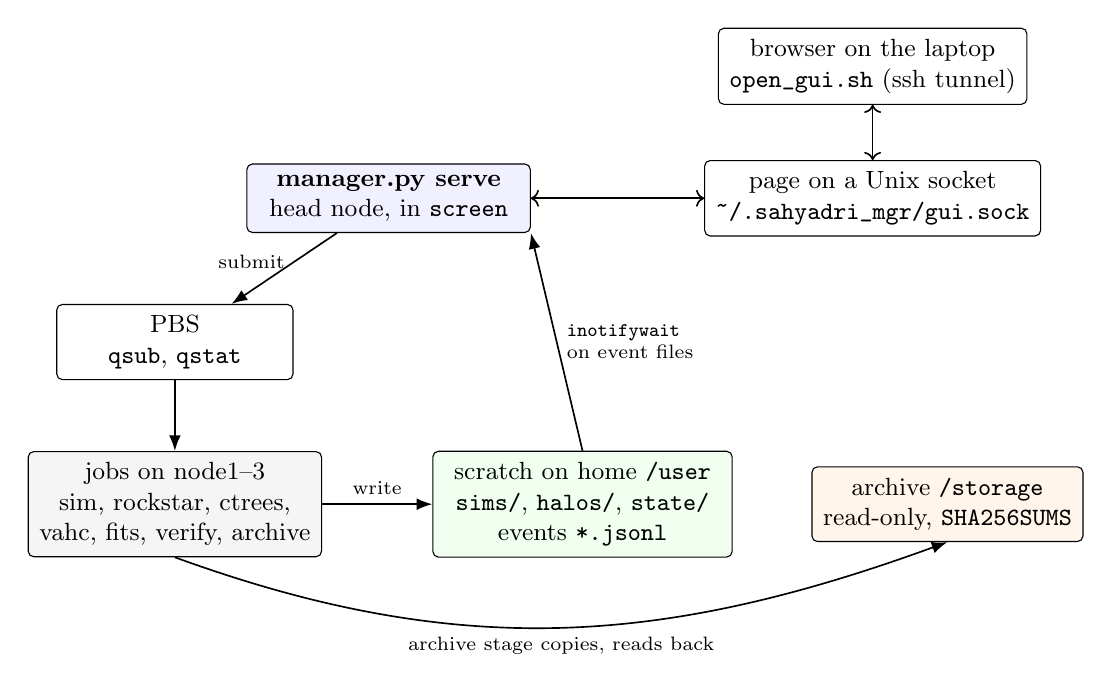
\begin{tikzpicture}[font=\small, node distance=6mm and 9mm,
  box/.style={draw, rounded corners=2pt, align=center, inner sep=4pt, fill=#1},
  box/.default=white, arr/.style={-{Latex[length=2mm]}, semithick}]
  \node[box=blue!6, minimum width=36mm] (mgr) {\textbf{manager.py serve}\\ head node, in \code{screen}};
  \node[box, below left=9mm and -6mm of mgr, minimum width=30mm] (pbs) {PBS\\ \code{qsub}, \code{qstat}};
  \node[box=black!4, below=9mm of pbs, minimum width=30mm] (jobs) {jobs on node1--3\\ sim, rockstar, ctrees,\\ vahc, fits, verify, archive};
  \node[box=green!6, right=14mm of jobs, minimum width=38mm] (scr) {scratch on home \code{/user}\\ \code{sims/}, \code{halos/}, \code{state/}\\ events \code{*.jsonl}};
  \node[box=orange!8, right=10mm of scr, minimum width=30mm] (arc) {archive \code{/storage}\\ read-only, \code{SHA256SUMS}};
  \node[box, right=22mm of mgr, minimum width=30mm] (sock) {page on a Unix socket\\ \code{~/.sahyadri_mgr/gui.sock}};
  \node[box, above=7mm of sock, minimum width=30mm] (mac) {browser on the laptop\\ \code{open_gui.sh} (ssh tunnel)};
  \draw[arr] (mgr) -- node[left, font=\scriptsize, pos=0.4] {submit} (pbs);
  \draw[arr] (pbs) -- (jobs);
  \draw[arr] (jobs) -- node[above, font=\scriptsize] {write} (scr);
  \draw[arr] (jobs.south) to[out=-20, in=-160] node[below, font=\scriptsize] {archive stage copies, reads back} (arc.south);
  \draw[arr] (scr.north) -- node[right, font=\scriptsize, align=left] {\code{inotifywait}\\ on event files} (mgr.south east);
  \draw[arr, <->] (mgr) -- (sock);
  \draw[arr, <->] (sock) -- (mac);
\end{tikzpicture}
\caption{Components. The manager submits every job and learns what happened from the event files that the jobs
write to the scratch area on home. The scratch area is a disk of the head node, so \code{inotifywait} sees these
writes as they happen. The archive stage runs as a PBS job; only the deletion of scratch data is done by the
manager itself, after approval on the page.}
\label{fig:design}
\end{figure}

Figure~\ref{fig:design} shows the parts. Four choices shape the design.

\paragraph{The state lives in files.}
Every job appends JSON lines to its own event file,
\[ \code{<SCRATCH>/state/<stem>/r<real>/events/<time>.<stage>.<job>.jsonl} : \]
\code{start}, \code{end} with the exit code, \code{snap_ready} for each output once all its files are complete in
scratch, and one line per finished product (\code{rockstar_done} with the batch's snapshot range,
\code{ctrees_done}, \code{vahc_done}, \code{fits_done}, \code{verify_done}, \code{archive_done}). The manager writes
only \code{manager.json} per run (submitted jobs, failures, approvals, queue entry) and its own configuration
\code{~/.sahyadri_mgr/config.json}. Stopping and restarting the manager loses nothing; on start it reads all
event files and continues. This was used many times during the tests, to load new code.

\paragraph{It waits for events, not by polling.}
\code{/user} is exported by the head node, so a single \code{inotifywait -m -r} on the state directories reports
every event line written by any compute node. The manager acts when a line arrives. \code{qstat} runs only at
start, every 30 minutes (\code{heartbeat_s}), from the page's \emph{Check now} button, and about 3 minutes after
a job seems to have disappeared. A job that leaves PBS without an \code{end} line (killed, node failure) is
reported as vanished.

\paragraph{Clocks are not trusted.}
The compute nodes' clocks run behind the head node: node2 by about 81\,s, node3 by about 182\,s and node1 by about
3\,min, and \code{/storage}'s file times by about 15\,min (measured by short PBS jobs printing \code{date} and
writing a file on each node, compared with the head node's \code{date} and the files' modification times).
Ordering decisions (``did verify pass \emph{after} the last vahc?'', ``is there an archive newer than this
verify?'') therefore use PBS job numbers, which only increase, or the modification times of files on the same
server. Durations quoted in this report are differences of two time stamps written by the same job on the same
node, so the offsets cancel.

\paragraph{Deletion needs a person.}
Everything up to and including the archive is automatic. Removing scratch data is not: the page offers
\emph{Move scratch data to the trash} only after the archive passed, and \emph{Purge} only after a second
approval, typed as the run name.

\section{The pipeline under the manager}

\begin{table}[t]
\centering\small
\begin{tabularx}{\linewidth}{@{}l >{\raggedright\arraybackslash}p{5.2cm} >{\raggedright\arraybackslash}X@{}}
\toprule
stage & started by the manager when & does \\
\midrule
sim & you press \emph{Submit}, or the queue's turn comes (Section~\ref{sec:queue}) &
  pkdgrav3, snapshots as \code{.pkc}; with \code{SIM_STAGING=1} written to the node's SSD and copied to home while
  the run continues; \code{snap_ready} per complete output \\
rockstar & \code{RS_BATCH_MIN} (10) consecutive snapshots after the last batch are ready, or the simulation ended &
  Rockstar on snapshots \code{A--B} (\code{--rs-snaps A-B}); reads the previous batch's halo files to link
  halos in time; at most \code{max_rockstar} such jobs over all runs \\
ctrees, vahc, fits, verify & Rockstar covers every snapshot & one \code{afterok} chain: merger trees; halo
  environment tables and P(k) (\code{run_addvalue.py}, \code{pk_measure.py}, \code{class_pk.py}); FITS with a
  read-back check; the checks of Section~\ref{sec:checks} \\
archive & verify passed after the last change & copies the kept files to \code{/storage} with SHA-256, reads every
  copy back with \code{O_DIRECT}, writes \code{MANIFEST.json} and \code{SHA256SUMS}, makes it read-only \\
trash, purge & you approve, twice & rename the run's scratch directories into \code{<SCRATCH>/.trash/}
  (undoable), then delete them \\
\bottomrule
\end{tabularx}
\caption{Stages and what starts them. A failed stage (exit code $\neq 0$ or vanished job) stops the run's
automation until you press \emph{Retry} (resubmit that stage; a Rockstar batch continues after its newest
finished snapshot) or \emph{Acknowledge}.}
\label{tab:stages}
\end{table}

Table~\ref{tab:stages} lists the stages. Two are new: \code{verify} and \code{archive}.

\subsection{Rockstar in batches}
Rockstar's temporal halo finding uses the halos of the previous snapshot. A batch starting at snapshot $A>0$ finds
them in the halo files that the previous batch wrote for snapshot $A-1$. The job script copies these back from the
node's local disk at the end of every batch, and links them at the start of the next. One detail cost two test
iterations: Rockstar names its binary halo files by the pkdgrav3 step (\code{halos_02126.*.bin}), but its
catalogues by the snapshot number (\code{out_100.list}). The job now converts between the two through the run's
snapshot list wherever it touches these files.

A batch takes all snapshots that are ready when it is submitted, so batches grow when Rockstar is the bottleneck.
With several runs and \code{max_rockstar} jobs already running, the run whose next ready snapshot has waited longest
(by the manager's clock) gets the next turn.

\subsection{The simulation queue}\label{sec:queue}
A run can be \emph{scheduled}: from the page, with \code{manager.py schedule <stem/rN> [--priority N] [--at "YYYY-MM-DD HH:MM"]},
or for many runs at once with \code{setup_production.py ... --schedule [N]}. The manager submits scheduled
simulations, lowest priority number first, then the earliest scheduled, while
\[
  n_\text{running} + n_\text{waiting in PBS} < \code{max_sim_running} \quad\text{and}\quad n_\text{waiting in PBS} < \code{max_sim_queued},
\]
after the \code{--at} time, and only if the run fits in scratch:
\[
  \text{free} - \text{estimate(this run)} - \textstyle\sum \text{still to be written by running simulations} - \code{scratch_reserve_gb} \ge 0 .
\]
The estimate is $1.1\times(1.15\times 10.5\,\text{B}\times N^3 \times n_\text{out} + 48\,\text{B}\times N^3\times \code{SIM_KEEPCHK})$:
every output in full, 15\,\% for halo products, the kept checkpoints, and 10\,\% margin. The reserve (default
2000\,GB) leaves room for other users of home. A simulation that stops cleanly at its wall time --- a checkpoint
was written and outputs are missing --- is queued again at priority $-1$, ahead of everything, and restarts from its
newest checkpoint, at most \code{max_sim_restarts} (5) times. A simulation that fails in any other way stops the run.

The limits are set on the page or with \code{manager.py limits key=value ...}; defaults
\code{max_sim_running=3}, \code{max_sim_queued=1}, \code{max_sim_restarts=5}, \code{max_rockstar=1}.

\subsection{What is kept}
\code{setup_production.py} writes the retention settings into each run's \code{run.conf}:

\begin{lstlisting}
KEEP_FULL_Z="0 0.5 1 2 3 5 7"   # full snapshots: the planned output nearest each redshift
KEEP_SUBSAMPLE_PCT=1             # % of the particles of every other snapshot (sum of leading SUBSAMPLES 1,4,9,...)
KEEP_HALO_TABLES="basic,extended,tens,vahc"
KEEP_TREES=1; KEEP_CHECKPOINT=0
ARCHIVE_FILE_MODE=0444; ARCHIVE_DIR_MODE=0555
\end{lstlisting}

\code{retention.py run.conf} prints the resolved plan (which snapshot numbers, which files). The archive also holds
each run's own copy of its cosmology files, \code{scales.txt}, the logs, the event files, and the P(k) files and plot.

\section{Checks before anything is deleted}\label{sec:checks}

\subsection{verify}
\code{verify_run.py} writes \code{verify.json} with one entry per check:
\begin{itemize}
  \item \textbf{snapshots}: every output has all its \code{.pkc} files complete (header, trailer, particle count),
    $N^3$ particles, the planned redshift, the subsamples and the potential. The kept full snapshots are also run
    through \code{pkc_check}, which confirms that every particle ID occurs exactly once;
  \item \textbf{subsample}: holds the configured fraction of the particles;
  \item \textbf{Rockstar}: every snapshot is covered by a batch that ended successfully;
  \item \textbf{trees}: present for every snapshot from the first with halos on;
  \item \textbf{vahc, tens, vpot}: the same halo IDs in the same order as the \code{.trees} catalogue;
  \item \textbf{FITS}: the FITS stage passed its read-back check, ran after the last vahc, and every kept table is present;
  \item \textbf{P(k)}: Section~\ref{sec:pk}.
\end{itemize}

\subsection{Power spectrum}\label{sec:pk}
The vahc stage builds a CIC density grid (\code{PP_GRID}$^3$) of every output with halos. From the same grid
\code{pk_measure.py} now also computes the matter power spectrum (CIC window deconvolved, no interlacing), and the
halo--matter and halo--halo spectra of host halos in five bins of $M_\text{vir}$ (100, 300, 1000, 3000 and
$\ge 10^4$ particles), with $b_{hm}(k) = P_{hm}/P_{mm}$ and a large-scale $b_1$. Outputs without halos get a
density-only pass. \code{class_pk.py} computes CLASS 3.4.2 linear and halofit spectra at every output redshift,
with the production CLASS settings (\code{config/transfer/class_template_As.ini}), and the linear growth $D(z)$ of
matter + curvature + $(w_0, w_a)$ dark energy \emph{without radiation}, which is what pkdgrav3 integrates.

The checks use the bins with $k \le \code{PK_KLIN} = 0.1\,h/\text{Mpc}$:
\begin{description}
  \item[absolute] $R = \langle P_{mm}/P_\text{ref}\rangle_\text{modes}$ with
    $P_\text{ref}(k,z) = P_\text{CLASS}(k, z_\text{start})\,[D(z)/D(z_\text{start})]^2 \times P_\text{halofit}/P_\text{lin}$.
    Fails if $|R-1| > 4\sigma + 0.02$, $\sigma = \sqrt{2/N_\text{modes}}$ (cosmic variance). This catches
    normalisation, unit and growth errors, not the realisation's own scatter.
  \item[growth] $G = \langle [P(z)/P(z_0)] / [P_\text{ref}(z)/P_\text{ref}(z_0)] \rangle_\text{modes}$ against
    the first output $z_0$, over bins with $\Delta^2_\text{lin}(k,z) = k^3P_\text{lin}/2\pi^2 \le 0.01$. The same
    modes at both times, so the realisation's scatter cancels. Fails if $|G-1| > 0.03$.
  \item[IC table] CLASS at $z_\text{start}$ against the table the initial conditions were made from. Fails above 2\,\%.
  \item[reported] the ratio to CLASS at $z$ itself (which includes radiation: at $z=0$ CLASS gives
    $\sigma_8 = 0.8227$, the no-radiation growth from the same $z=49$ spectrum $0.8305$), and $b_1$ per mass bin.
\end{description}

Two choices here came from failures in the tests (Section~\ref{sec:bugs}). The spectra are not corrected for
shot noise: the particles start on a lattice, and on these scales their discreteness noise is far below the
Poisson $1/\bar n$. And the growth check uses only bins that are still nearly linear, because a bin of 6--12 modes
moves by $(2\text{--}3)\,\Delta^2_\text{lin}$ through mode coupling, with either sign.

\subsection{archive}
\code{archive_run.py} refuses unless verify passed after the last change to any kept file (by file times on the
scratch server). It copies each file while computing its SHA-256, reads every copy back from disk with
\code{O_DIRECT} (so the page cache cannot hide a bad write) and compares, writes \code{MANIFEST.json} and
\code{SHA256SUMS}, and sets the modes to 0444/0555. Its parent directories are made traversable for other users.
\code{cd <archive> && sha256sum -c state/<stem>/r<real>/SHA256SUMS} re-checks it at any time.

\subsection{Trash and purge}
\emph{Move to trash} first checks that no job of the run is active; that verify passed and an archive passed after
it; that every manifest entry is in the archive with the right size and checksum; and that every currently kept
file is in the manifest and unchanged since (size and modification time). Then it renames \code{sims/<stem>/r<real>}
and \code{halos/<stem>/r<real>} into \code{<SCRATCH>/.trash/}, which is instant and can be undone. \emph{Purge}
re-checks the archive and deletes the trash directory; it deletes nothing outside \code{<SCRATCH>/.trash/}.

\section{How to use it}

\subsection{Start the manager (once, on the pawna head node)}
\begin{lstlisting}
cd /user/$USER/sahyadri_rm/sahyadri-sandbox          # a clone on branch run-manager
tools/sahyadri_manager/start_manager.sh              # detached screen session "sahyadri_mgr"
tools/sahyadri_manager/start_manager.sh status       # running? plus the last log lines
tools/sahyadri_manager/start_manager.sh stop         # safe at any time: the state is in files
\end{lstlisting}
The log is \code{~/.sahyadri_mgr/manager.log}. To survive a reboot of the head node, add this line with
\code{crontab -e} (not done yet):
\begin{lstlisting}
@reboot <repo>/tools/sahyadri_manager/start_manager.sh
\end{lstlisting}

\subsection{Set up and queue runs}
\begin{lstlisting}
cd scripts/pkdgrav3_pipeline/production
# 4 realisations of the default cosmology, 2048^3 particles in 200 Mpc/h, queued at priority 0
python setup_production.py --cosmo default --N 2048 --L 200 --real 1-4 --schedule
# r1 of every variation cosmology, after those (higher number = later)
python setup_production.py --cosmo 'var_*' --N 2048 --L 200 --real 1 --schedule 5
# a single run, registered but not queued: submit it from the page
python setup_production.py --cosmo default --N 512 --L 200 --real 7
tools/sahyadri_manager/manager.py add <scratch>/sims/Sahyadri_L200N512/default512/r7/run.conf
\end{lstlisting}
\code{--cosmo} takes a name, a comma list, shell patterns or \code{all} (files
\code{production/cosmologies/<name>.cosmo}). Each realisation gets its own seed from \code{config/sims/seeds.txt}
(249 seeds); the same realisation number has the same seed in every cosmology. Other options: \code{--root}
(scratch, default \code{/user/\$USER/sahyadri_scratch}), \code{--archive} (default
\code{/storage/\$USER/sahyadri_sims}), \code{--keep-full-z}, \code{--keep-pct}. Only \code{default.cosmo} exists so
far; the variations used on pegasus need their \code{.cosmo} files (parameters and a CLASS table at $z=49$) first.

\subsection{Watch and act from the laptop}
\begin{lstlisting}
tools/sahyadri_manager/open_gui.sh           # ssh tunnel to the page's socket, opens http://localhost:8765
\end{lstlisting}
The page is served on the Unix socket \code{~/.sahyadri_mgr/gui.sock}, in a directory of mode 0700, so other users
of the head node cannot reach it; actions need a custom header, so another web page open in the same browser cannot
trigger them. Closing the laptop closes only the page. Figure~\ref{fig:page} shows it during the tests. For each run
it shows the phase, a strip with one cell per output (planned, written, halos found, kept in full), the stages with
their jobs, and fold-out panels: jobs now in PBS, the verify checks, the power spectrum plot, the retention plan and
archive state, the deletion steps, the event lines, and the manager's actions. At the top are the free space on
scratch and archive, the queue with its limits, and \emph{Check now}.

The same actions from a shell on the head node:
\begin{lstlisting}
manager.py list | add <run.conf> [--paused] | remove <stem/rN>
manager.py schedule <stem/rN> [--priority N] [--at "2026-11-20 08:00"] | unschedule <stem/rN>
manager.py limits max_sim_running=3 max_sim_queued=1 max_rockstar=1 scratch_reserve_gb=2000
\end{lstlisting}

\begin{figure}[p]
\centering
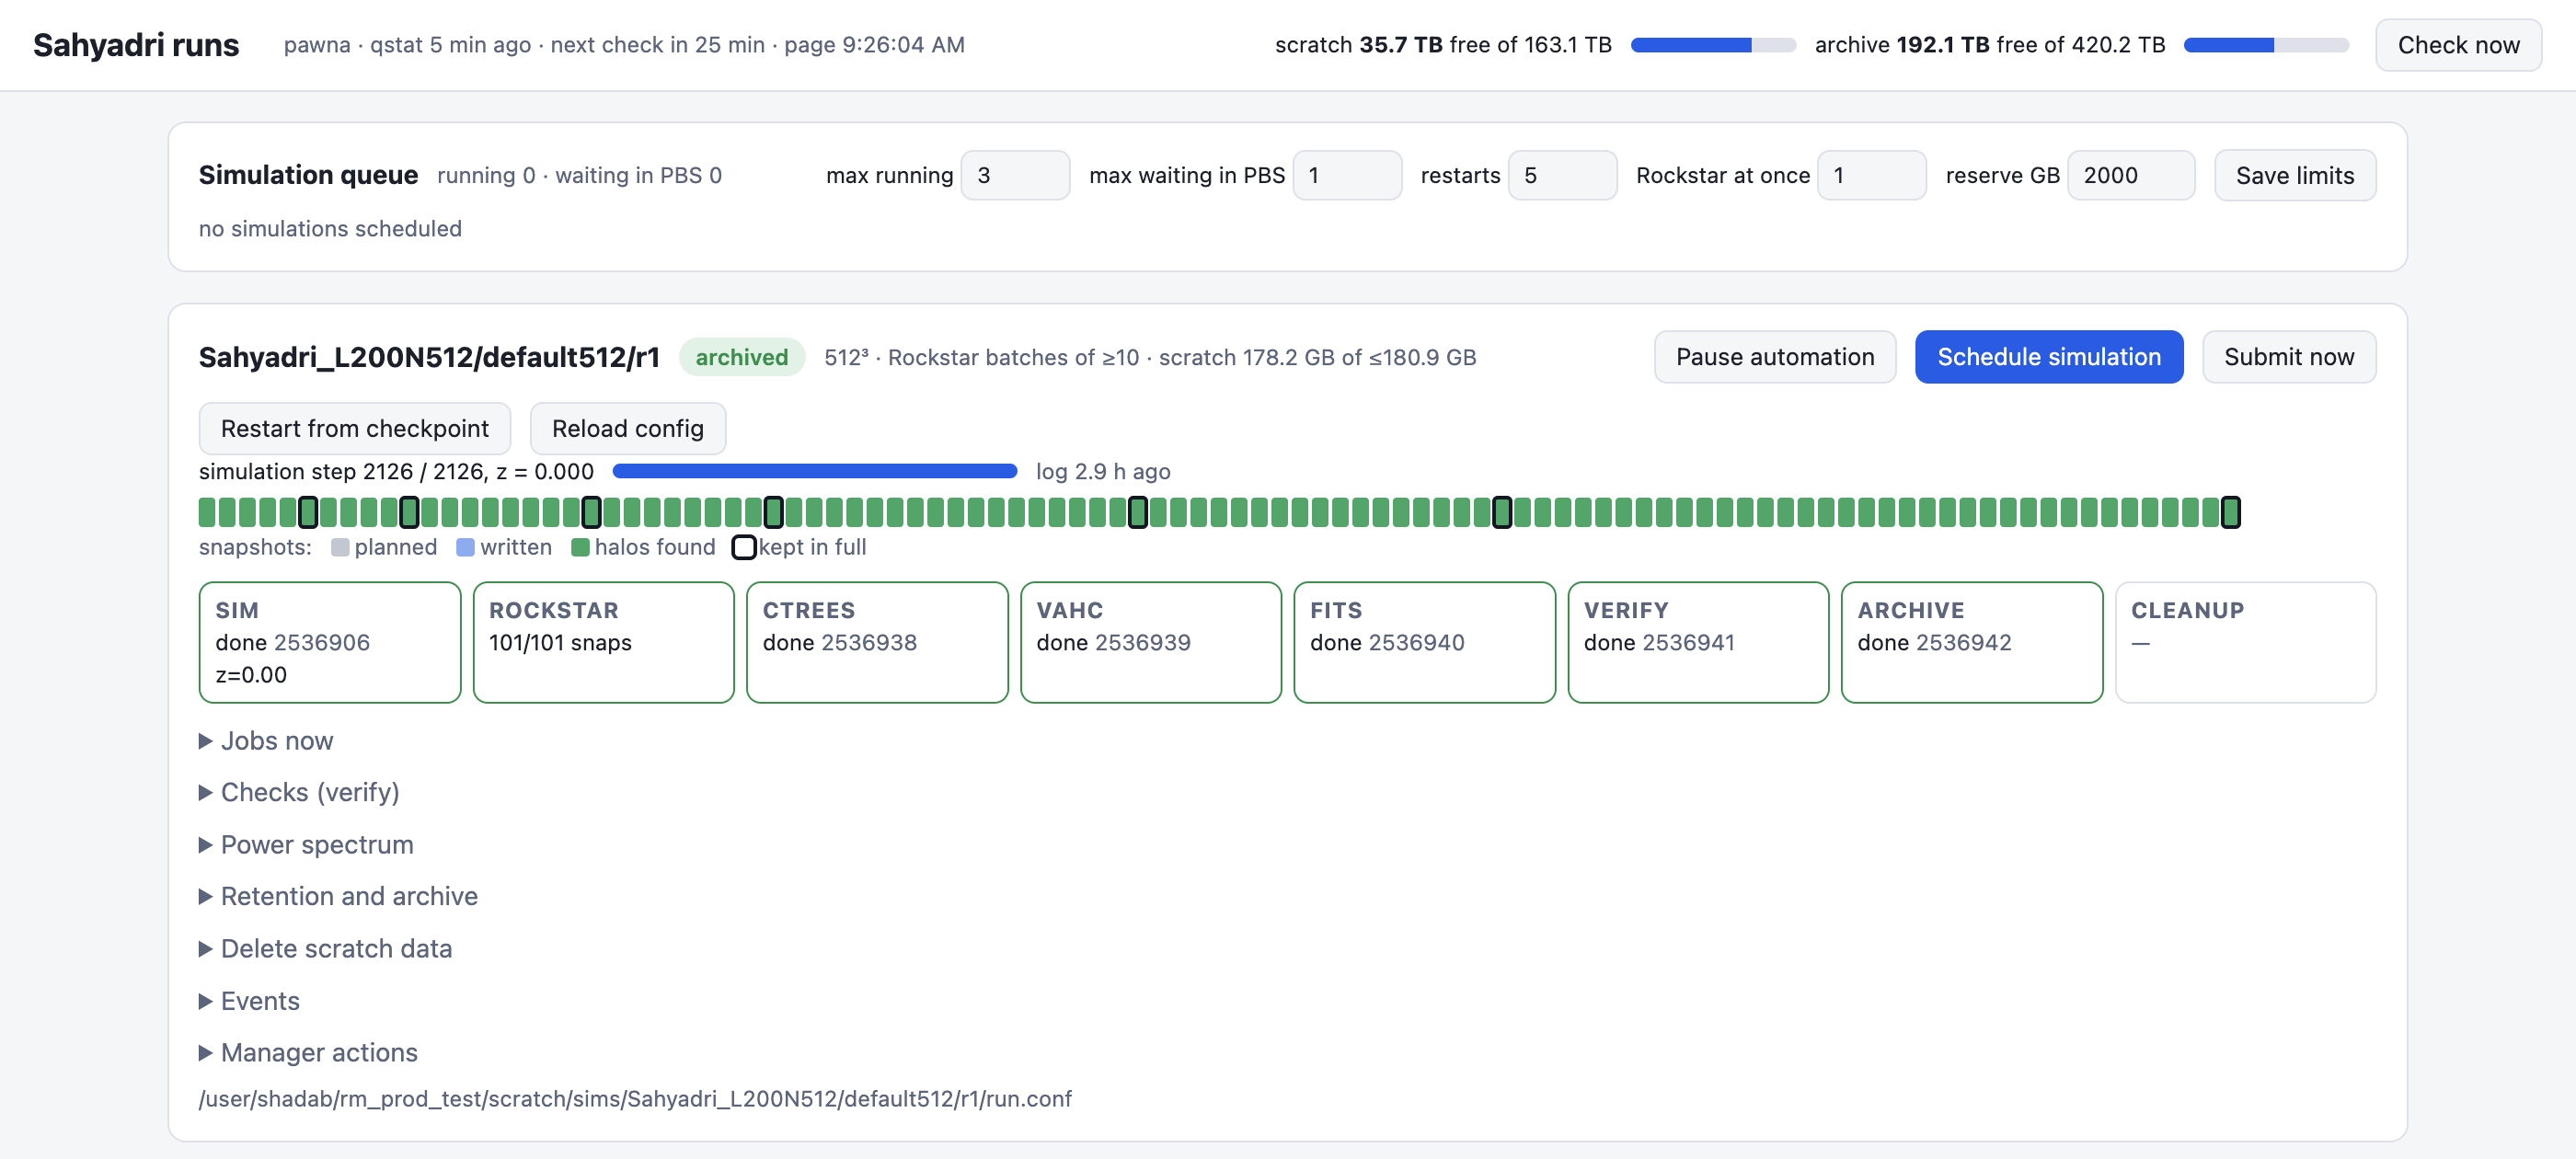
\includegraphics[width=\linewidth]{figures/sim_manager/manager_page.png}
\caption{The manager page after the production-size test, 13 November 2026, 09:26 IST (headless Chrome through the
ssh tunnel, cropped to the top of the page and one run). Top: free space on scratch and archive (each file system
once), and the simulation queue with its limits. Below: the archived $512^3$ run. Its line of 101 squares shows each
output's state (planned, written, halos found; outlined: kept in full), the eight boxes the stages with their PBS
jobs, and the folded sections the checks, the P(k) plot, the retention list and the deletion controls.}
\label{fig:page}
\end{figure}

\subsection{When something fails}
A failed job turns the run red and stops its automation. The job's log is linked on the page. After fixing the
cause, \emph{Retry} resubmits the failed stage: a Rockstar batch with its snapshot range, a post-processing stage
with the rest of its chain, or the archive. A failed simulation is only acknowledged by \emph{Retry};
\emph{Restart from checkpoint} continues it. \emph{Acknowledge} clears the failure
without resubmitting, for example after doing the step by hand. \emph{Pause automation} holds a run without
touching its jobs.

\section{Tests}\label{sec:tests}

All tests ran on pawna between 12 and 13 November 2026 under one manager instance on the head node, with jobs on
node1--3. \textbf{How the numbers were measured.} Stage durations are the difference between the \code{start} and
\code{end} event lines that each job writes, both stamped by the same job on its own node, so the clock offsets
between machines cancel. Archive sizes and file counts are from each run's \code{MANIFEST.json}. Rockstar batch
ranges are from the \code{rockstar_done} lines. Event times quoted as ``at hh:mm'' are on the node's clock, which
runs 1.5--3 minutes behind the head node. The numbers were collected with a script
(\code{test_summary.py}, run on the head node) that reads the event files and manifests of every test run.

\subsection{Logic tests at $64^3$}
{\sloppy Nine realisations of \code{Sahyadri_L100N64/default64} ($64^3$ particles, $100\,h^{-1}$Mpc, 101 outputs,
\code{PP_GRID}=64), scratch \code{/user/shadab/rm_test/scratch}, archive
\code{/storage/shadab/pipeline_test/rm_test_archive}.
Each test was chosen to exercise one part of the manager:\par}

\begin{description}
  \item[r1] the full chain once, then the deletion steps: the refusal when a kept file changed after the archive
    (a modification time moved by 1\,s, and separately one truncated to whole seconds, were both caught), trash,
    undo, trash again, purge. \code{sha256sum -c} on the archive passed before and after the purge.
  \item[r2] Rockstar batches while the simulation runs: the simulation wrote its outputs over 3.5\,min, and the
    manager submitted batches 0--9 and 10--30 during it and 31--100 after it. Every batch reported all its snapshots
    successful and read the previous batch's halo files.
  \item[r3--r5] three simulations at once (submitted together) with \code{max_rockstar=1}: Rockstar ran
    r3 0--9 $\to$ r4 0--29 $\to$ r5 0--100 $\to$ r3 10--100 $\to$ r4 30--100, one at a time; on the head node's
    clock each Rockstar job started about 1\,s after the previous one ended. Each run went on to its archive
    independently. Before this, the space check was tested by raising \code{scratch_reserve_gb} above the free
    space: submission was refused with the numbers (\code{scratch ...: 35.8 TB free; this run needs up to 361.8 MB,
    running simulations 0 B more, reserve 36.4 TB -> 550.2 GB SHORT}); with the reserve set back, the three were
    submitted.
  \item[r6--r9] the simulation queue with \code{max_sim_running=2}, \code{max_sim_queued=1}: r9 at priority 0 with
    a 1-minute wall time, r8 at priority 1 with \code{--at 01:27}. Never more than two simulations ran. r9 stopped
    at its wall time four times, was queued again at priority $-1$ each time and restarted from its newest
    checkpoint, and finished in its fifth job. r8 was submitted at 01:27:01. Scheduling r7 while its simulation
    ran was refused.
  \item[r6, r8] the P(k) stage and checks: first by hand on r6 (paused, so its archive stayed untouched), then
    inside the pipeline on r8, whose first verify failed (shot-noise subtraction, Section~\ref{sec:bugs}) and
    passed on \emph{Retry} after the fix.
\end{description}

\begin{table}[t]
\centering\small
\begin{tabular}{@{}l r l r r r r r r r@{}}
\toprule
run & sim & Rockstar batches (s) & ctrees & vahc & fits & verify & archive & MB & files \\
\midrule
r1 & 336 & 0--100: 698$^a$          & 48 & 227 & 44 & 30 & 49 & 59.3 & 537 \\
r2 & 250 & 0--9: 55, 10--30: 137, 31--100: 515 & 55 & 98 & 19 & 5 & 52$^b$ & 59.0 & 545 \\
r3 & 242 & 0--9: 55, 10--100: 652    & 49 & 130 & 36 & 7 & 53 & 58.1 & 531 \\
r4 & 243 & 0--29: 183, 30--100: 534  & 47 & 84 & 20 & 5 & 63 & 58.6 & 527 \\
r5 & 242 & 0--100: 672               & 52 & 104 & 21 & 7 & 45 & 58.4 & 529 \\
r6 & 233 & 0--9: 55, 10--100: 636    & 50 & 73 & 20 & 5 & 51 & 58.4 & 531 \\
r7 & 233 & 0--32: 201, 33--100: 495  & 50 & 72 & 19 & 25 & 238 & 59.1 & 531 \\
r8 & 242 & 0--100: 696               & 49 & 85 & 53 & 9$^c$ & 57 & 60.4 & 634 \\
r9 & 341$^d$ & 0--100: 683           & 49 & 71 & 20 & 8 & 44 & 59.2 & 557 \\
\bottomrule
\end{tabular}
\caption{The $64^3$ runs: duration of each stage in seconds (successful job), and the archive. Simulations: 16 cores, staged
I/O; Rockstar: 8 cores. $^a$ after two failed attempts (bugs 2 and 3).
$^b$ second attempt (bug 6). $^c$ second attempt, after the shot-noise fix; r8 is the first run archived with
P(k) files (105 files, 2.0\,MB). $^d$ five jobs, 83+78+79+80+21\,s: four stops at the 1-minute wall time and
the final one. The same stage takes up to 3 times longer in one run than in another (vahc 71--227\,s); the jobs ran on
different nodes, one of which also ran the $1024^3$ production simulation.}
\label{tab:t64}
\end{table}

Table~\ref{tab:t64} lists the stage durations. At $64^3$ every stage is dominated by start-up costs, so these are
tests of the logic, not of performance.

\subsection{Production-size test: $128^3$ and $512^3$}\label{sec:prod}
{\sloppy Three runs of $200\,h^{-1}$Mpc boxes with production settings (\code{PP_GRID}=512, full snapshots kept
at $z=0, 0.5, 1, 2, 3, 5, 7$, a 1\,\% subsample of the others, all halo tables and trees):
\code{Sahyadri_L200N128/default128} r1 and r2, and \code{Sahyadri_L200N512/default512} r1. Scratch
\code{/user/shadab/rm_prod_test/scratch}, archive \code{/storage/shadab/pipeline_test/rm_prod_test_archive}.
All three were registered with one manager and scheduled together; nothing was done by hand except the
\emph{Retry} described below. The $512^3$ run and $128^3$ r1 have the same seed (12345678).\par}

\begin{table}[t]
\centering\small
\begin{tabular}{@{}l r l r r r r r r r@{}}
\toprule
run & sim & Rockstar batches (s) & ctrees & vahc & fits & verify & archive & GB & files \\
\midrule
$128^3$ r1 & 614 & 0--19: 146, 20--100: 761 & 79 & 5356 & 42 & 15 & 75 & 0.37 & 668 \\
$128^3$ r2 & 524 & 0--10: 81, 11--56: 396, 57--100: 412 & 73 & 4382 & 37 & 13$^a$ & 71 & 0.37 & 674 \\
$512^3$ r1 & 15762 & 11 batches, 56--379 each, 3268 in all & 3158 & 3130 & 1754 & 343 & 1105 & 23.3 & 778 \\
\bottomrule
\end{tabular}
\caption{The production-size runs: duration of each stage in seconds (measured as for Table~\ref{tab:t64}).
Cores: simulation 64 ($128^3$) and 96 ($512^3$); Rockstar 16 and 64; vahc 16 cores with 4 snapshots in parallel
and 32 cores with 8; FITS 8 and 16. $^a$ second attempt; the first failed the growth check (bug 11).}
\label{tab:tprod}
\end{table}

\paragraph{Timeline of the $512^3$ run.} (Node clock of the simulation's node, node3.) The simulation started at
02:08 on 96 cores and wrote its 101 outputs between 02:31 and 06:30 (2126 steps, 4.4\,h). The manager submitted
Rockstar in batches of ten snapshots as they appeared, about every 21 minutes; each batch took 3.4--6.3\,min, so
Rockstar kept pace with the simulation and was never more than one batch behind. The batch time grows from 201\,s
(snapshots 0--9) to 373--379\,s (70--99) as the halo count grows (248\,581 halos at $z=0$). The last batch
(snapshot 100 alone, 56\,s) was submitted 7\,min after the simulation ended, and the chain ctrees $\to$ vahc
$\to$ fits $\to$ verify one minute after that. Verify passed at 09:02, the archive was submitted at 09:03 and
finished after 18\,min. From the start of the simulation to the archived run took 7.2\,h, of which 2.9\,h
came after the simulation (2.65\,h of job time, the rest waiting for submission and PBS): consistent-trees (53\,min, on 2 cores) and vahc (52\,min) are the longest.

\paragraph{Scratch use and the archive.} The run used 178.2\,GB of scratch against the manager's estimate of at
most 180.9\,GB, measured by the manager's own walk of the run's directories, and 128\,GB of it is the simulation
directory (\code{du}). The archive holds 23.3\,GB in 778 files: 8.3\,GB for the seven full snapshots, 1.3\,GB
subsamples, 10.1\,GB halo tables, 3.6\,GB trees, 2.6\,MB P(k). Copying, reading back and checksumming took 1105\,s,
21\,MB/s overall, close to the 23--31\,MB/s write rate measured for \code{/storage} before.

\paragraph{Checks of the $512^3$ run.} \code{pkc_check} passed on all seven full snapshots (17--21\,s each); the
subsample fraction is 1.0005\,\%; trees exist from snapshot 2 on; 795 FITS files passed. The CLASS table at
$z=49$ agrees with the initial-conditions table to 0.11\,\% (median ratio 1.00008). The growth check used 122
modes per output and gave $G = 0.987$--0.999, within the 3\,\% limit. The absolute check gave $R=0.73$--0.78 against a
limit of $|R-1| \le 0.53$ for these modes; the low value is this realisation's large-scale power, not an error:
$128^3$ r1, with the same seed, gave $R = 0.73$--0.78 as well, and its per-bin ratios at the lowest $k$
(0.60, 1.38, 0.83, 1.32) are those of the $512^3$ run (Figure~\ref{fig:pk512}, middle). At $z=0$ the large-scale
halo bias of the five mass bins is $b_1 = 0.80, 0.91, 1.09, 1.43, 1.99$ (37\,865 to 575 halos).

\begin{figure}[t]
\centering
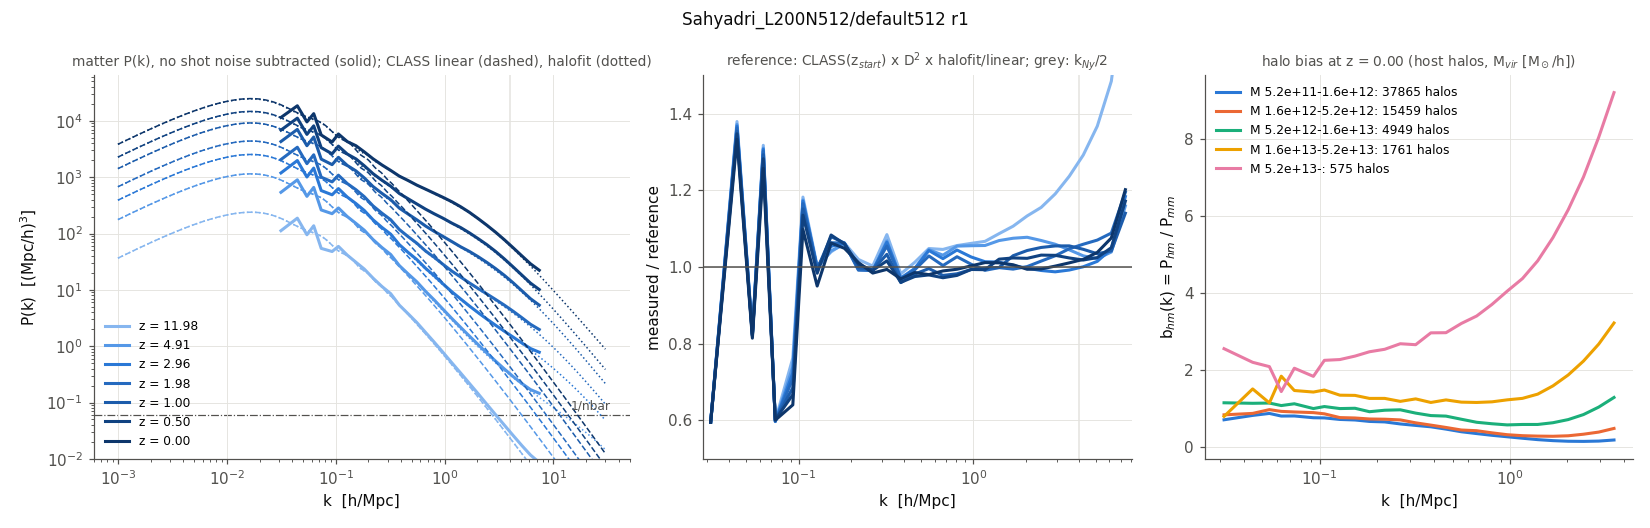
\includegraphics[width=\linewidth]{figures/sim_manager/pk_512.png}
\caption{The P(k) summary that the pipeline writes for every run (\code{pk/pk_summary.png}), here
\code{Sahyadri_L200N512/default512} r1. Left: measured $P_{mm}$ at seven redshifts with CLASS linear (dashed) and
halofit (dotted). Middle: ratio to the reference $P_\text{ref}$; the scatter at $k < 0.1\,h$/Mpc is the same at
every redshift, as it must be for the realisation's own modes, and above $k\approx1\,h$/Mpc the $z=12$ curve rises
from the discreteness of the lattice start. Right: $b_{hm}(k)$ for the five halo mass bins at $z=0$.}
\label{fig:pk512}
\end{figure}

\paragraph{The $128^3$ runs.} These ran next to the $512^3$ run on the same nodes. Their vahc stage took
73--89\,min, longer than at $512^3$: its cost is set by the $512^3$ density grid and the tidal field at every
output (about 200\,s per output), not by the particle number, and the $128^3$ runs had half as many outputs in
parallel (4 instead of 8). For small runs, \code{PP_GRID}=256 would be enough. r2's first verify failed the
growth check at $z<1.24$ with $G = 1.03$--1.04. That was a check that was too tight for bins of 6--12 modes (bug 11);
after the change, \emph{Retry} passed in 13\,s and the manager archived the run.

\paragraph{Summary.} Every stage ran without intervention at $512^3$. The scratch estimate held. Rockstar in
batches kept up with a 96-core simulation. The archive is limited by \code{/storage}'s write rate. The only failure was a check that
was too strict.

\section{Problems found by the tests}\label{sec:bugs}

\begin{table}[h]
\centering\small
\begin{tabularx}{\linewidth}{@{}r X X l@{}}
\toprule
& symptom & cause and fix & commit \\
\midrule
1 & manager idle for 20\,min after a finished simulation & snapshot steps such as \code{00124} written as JSON numbers with leading zeros (invalid); the manager skipped all 202 lines. Now written as strings; old lines still read & \code{429ad2a} \\
2 & order checks unreliable & compute nodes 1.5--3\,min and \code{/storage} 15\,min behind the head node; ordering now by PBS job numbers or same-server file times & \code{429ad2a} \\
3 & Rockstar batch reported failed although Rockstar succeeded & copy-back kept the last snapshot in \code{restart.cfg} (99), not the batch's last (100) & \code{e6dad40} \\
4 & no halo file ever copied back & Rockstar names halo files by pkdgrav3 step, catalogues by snapshot number; conversion through the snapshot list. The same mistake is in the held Rockstar job of the $1024^3$ production run (other branch); it matters there only for a Rockstar restart & \code{90e563b} \\
5 & archive not readable by other users & parent directories created 0700; now made traversable & \code{f92deca} \\
6 & manager page froze for 35--70\,s & checks reading the slow \code{/storage} ran in the event loop; now in a worker thread & \code{083bfa2} \\
7 & r2's archive refused to overwrite r1's read-only \code{cosmology.txt} & cosmology files and \code{scales.txt} shared by all realisations and rewritten by each; every run now keeps its own copies & \code{106388a} \\
8 & r7's simulation would have been submitted twice & a run could be scheduled while its simulation was running, and finished runs stayed queued; both refused/dropped now & \code{0bba128} \\
9 & r8 verify: growth 1.04--1.07 above linear at $z=9.5$--6.5 & $1/\bar n$ subtracted from $P(k)$; for lattice-started particles the discreteness noise on these scales is far below Poisson (subtraction removed 7\,\% of the $z=12$ power at $k=0.063\,h$/Mpc); raw $P_{mm}$ used now & \code{54f4e0f} \\
10 & r6 verify: growth 12\,\% below linear at $z=0$, $k\approx0.09\,h$/Mpc & mode coupling: check only bins with $\Delta^2_\text{lin}\le0.05$ & \code{9093218} \\
11 & 128$^3$ r2 verify: growth 1.03--1.04 at $z<1.24$ & bins of 6--12 modes move by $(2$--$3)\,\Delta^2_\text{lin}$ either way (measured: $+6$, $-6$, $+10$\,\% at $\Delta^2_\text{lin}=0.02$--0.04); limit lowered to 0.01 & \code{fabac12} \\
12 & purged run shown with a red configuration error & its \code{output_steps.txt} went with its directory; not an error after trash/purge & \code{bdd0238} \\
13 & no progress line for a running simulation & \code{run.log} linked only at the end of the job; manager reads the newest \code{run.<job>.log}, the job links it at the start & \code{fd51ed5} \\
14 & finished $512^3$ simulation still shown with a speed and an end time & rate and estimate now shown only before the last step & \code{3686bf4} \\
\bottomrule
\end{tabularx}
\caption{Problems found during the tests, all fixed on \code{run-manager}.}
\label{tab:bugs}
\end{table}

Bugs 1, 2 and 8 would have caused silent misbehaviour at scale (a run never post-processed; an archive judged
against the wrong verify; a second simulation writing into the first one's directory). Bugs 9--11 were in the new
P(k) checks themselves: the checks failed on correct simulations. Each failure was investigated down to the bins
before the check was changed, and the reasons are written next to the code.

\section{Open items}

\begin{itemize}
  \item \textbf{Merge.} Everything is on the branch \code{run-manager}; it is not merged into \code{master}.
  \item \textbf{Variation cosmologies.} Only \code{default.cosmo} exists. The pegasus variations need
    \code{.cosmo} files (parameters and a CLASS table at $z=49$) before \code{--cosmo 'var_*'} can be used.
  \item \textbf{Reboot.} The \code{@reboot} crontab line for the manager is not installed. After a reboot of the
    head node the manager has to be started by hand; it then catches up from the event files.
  \item \textbf{Untested at $2048^3$.} The archive copies with one Python process to \code{/storage}, measured at
    23--31\,MB/s for writes: about 1.2\,TB per $2048^3$ run would take 11--15\,h plus about 1.5\,h to read back,
    within the 72\,h limit but not measured. verify runs \code{pkc_check} on 7 full snapshots of about 90\,GB each.
    Rockstar's halo files carried from batch to batch grow with $N$.
  \item \textbf{Low-$k$ bins.} With four realisations, the power in the bin at $k=\sqrt2\,k_f$ is on average
    $1.38\pm0.2$ times the reference ($0.43$--$1.93$ in single runs), and at $\sqrt3\,k_f$ $0.84\pm0.25$. This is
    consistent with cosmic variance (each bin has 4--6 independent modes) but worth re-checking when more
    realisations exist.
  \item \textbf{Aliasing.} The P(k) estimator does not interlace; above $k_\text{Ny}/2$ the spectra are not used.
  \item \textbf{Clocks.} The compute nodes and \code{/storage} drift by minutes against the head node; the
    administrators may want to fix NTP. The manager does not depend on it.
\end{itemize}



\end{document}
